\documentclass[a4paper,10pt,twoside]{article}
\usepackage[left=1in, right=1in, top=1in, bottom=1in]{geometry} % Page margins
\usepackage{graphicx}
\usepackage{hyperref}
\usepackage{booktabs}
\usepackage[dvipsnames]{xcolor}
\usepackage{caption}
\usepackage{listings}
%\usepackage{lineno}  % Enable line numbers on both sides
\usepackage{blindtext}
\usepackage{fancyhdr}  % Enable page numbering in header/footer
\usepackage{multirow}
\usepackage{longtable,booktabs,array}
\usepackage{calc}
\usepackage[
includehead,
nomarginpar,% We don't want any margin paragraphs
textwidth=10cm,% Set \textwidth to 10cm
headheight=25pt,% Set \headheight to 25pt to accommodate the multiline header
]{geometry}
\usepackage{fancyhdr}
\usepackage{datetime2}

\usepackage[left, right]{lineno}  % Enable line numbers on both sides
\usepackage{etoolbox}  % Required for modifying commands
\preto{\newpage}{\resetlinenumber}
\preto{\pagebreak}{\resetlinenumber}
\linenumbers  % Enable line numbering globally
\modulolinenumbers[1]  % Number every line

\makeatletter
\def\makeLineNumberLeft{%
  \linenumberfont\llap{\hb@xt@\linenumberwidth{\LineNumber\hss}\hskip\linenumbersep}% left line number
  \hskip\columnwidth% skip over column of text
  \rlap{\hskip\linenumbersep\hb@xt@\linenumberwidth{\hss\LineNumber}}\hss}% right line number
\leftlinenumbers  % Ensure line numbers appear on the left
\makeatother



\urlstyle{same} % disable monospaced font for URLs
\hypersetup{
  hidelinks}

% Configure page numbers
\pagestyle{fancy}
\fancyhf{}  % Clear all header and footer fields
%... then configure it.
\fancyhead{} % clear all header fields
\fancyhead[RO,RE]{{\footnotesize \textsc{Netflix SDLC Analysis},in: (ed.): \LaTeX .\\  typeset \DTMnow}}

\fancyfoot[C]{Page \thepage}  % Centered page number at the bottom

\title{\textbf{Software Development Lifecycle (SDLC) Analysis of Netflix} \\ \large A Comparative Study of Different Models in Relation to Netflix’s Software Development}
\author{Delston Aaron Pereira \\ Nitte Mahalinga Adyantaya Memorial Institute of Technology \\ \text{\{delston.aaron@gmail.com, nnm23is044@nmamit.in\}}}
\date{}

\begin{document}

\maketitle
\begin{center}
    \url{https://github.com/delston-aaron/SDLC-real-world-analysis}
\end{center}

\begin{longtable}[]{@{}
  >{\raggedright\arraybackslash}p{(\columnwidth - 2\tabcolsep) * \real{0.1296}}
  >{\raggedright\arraybackslash}p{(\columnwidth - 2\tabcolsep) * \real{0.8704}}@{}}
\toprule()
\begin{minipage}[b]{\linewidth}\raggedright
\end{minipage}
Keywords: & \begin{minipage}[b]{\linewidth}\raggedright
SDLC, Netflix, AWS, Integration, Testing, Scalability, Requirements validation
\end{minipage} \\
\midrule()

Abstract: & Software development is an evolving discipline requiring structured approaches for building scalable, secure, and efficient systems. This report explores the Software Development Life Cycle (SDLC) models applicable to Netflix, a global leader in video streaming services. It provides a comparative analysis of SDLC methodologies, an overview of requirements engineering.
The study aims to offer insights into the selection of an appropriate SDLC model for large-scale cloud-based platform (Netflix for this report), emphasizing the waterfall, incremental development and spiral model approaches. The report also discusses challenges and strategies involved in requirements validation and software deployment at Netflix.
The findings in this document are based on extensive research, industry best practices, and insights from Netflix’s technology stack. I hope this report serves as a valuable resource for software engineers, architects, and researchers interested in the intersection of SDLC and requirements engineering methodologies and large-scale streaming platforms. This paper is followed by a conclusion and few considerations. \\
Publishing: & \begin{minipage}[t]{\linewidth}\raggedright
This paper is hosted on a GitHub repository, along with the
material used for preparing this research.
\end{minipage} \\
\bottomrule()
\end{longtable}

\tableofcontents
\newpage

\section{Introduction}
Netflix is one of the leading video streaming platforms globally, offering on-demand content to millions of users. The platform relies on a robust cloud-based infrastructure, primarily hosted on \textcolor{Blue}{Amazon Web Services (AWS)}. Given its large-scale nature, Netflix requires an efficient software development lifecycle (SDLC) to manage continuous updates, new features, and system stability.
This report conducts a comparative study of incremental development, spiral model, and waterfall model in relation to Netflix’s software development. It also explores requirements engineering, and the challenges faced.

\section{Overview of Netflix}
\subsection{System Overview}
Netflix provides subscription-based access to movies, TV shows, and original content. The system supports multiple devices, personalized recommendations, and high-quality video streaming with adaptive bitrate technology. It is an American subscription service providing video \textcolor{Blue}{on-demand} and \textcolor{Blue}{over-the-top} streaming. The service primarily distributes both original and acquired films and television shows from various genres, and it is available internationally in multiple languages.

\subsection{Technologies Used}
\begin{itemize}
    \item \textbf{Cloud Platform}: AWS (Amazon Web Services)
    \item \textbf{Architecture}: Microservices-based
    \item \textbf{Database}: NoSQL (DynamoDB, Cassandra), MySQL
    \item \textbf{Content Delivery}: AWS CloudFront, Open Connect
    \item \textbf{Programming Languages}: Java, Python, Node.js
    \item \textbf{DevOps}: Continuous Integration \& Continuous Deployment (CI/CD)
\end{itemize}
Netflix does use more technologies in every department. The ones mentioned above are just the major ones, powering the streaming platform in each individual component. Each of these component works seamlessly across the platform to provide users with a reliable stream. 

\begin{figure}[tbhp]
\centering
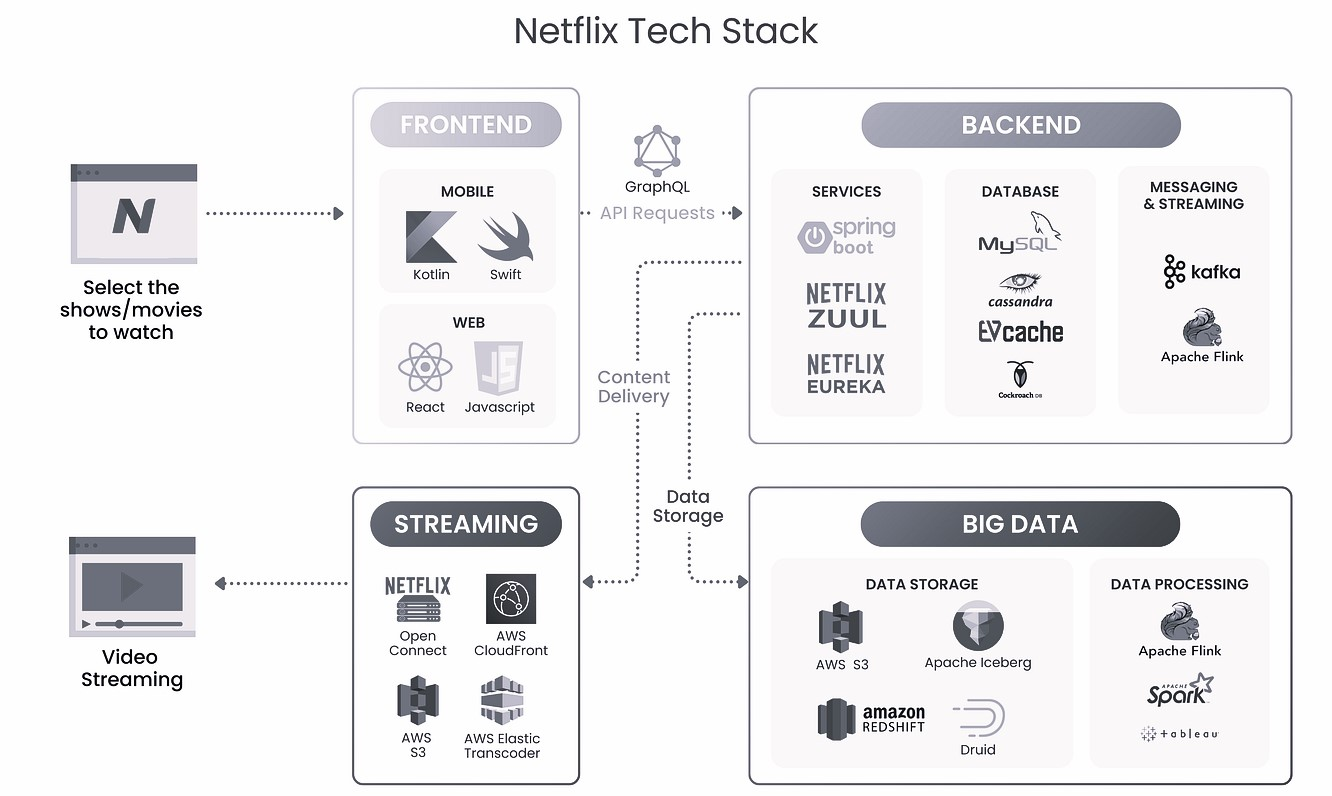
\includegraphics[width=.8\linewidth]{techstack-edited.jpg}
\caption{Figure 1- Represents the diverse tech stack}
\label{fig:techstack}
\end{figure}
\newpage

\section{Comparative Analysis of SDLC Models}
\subsection{\textcolor{Blue}{Waterfall Model}}
\begin{figure}[tbhp]
\centering
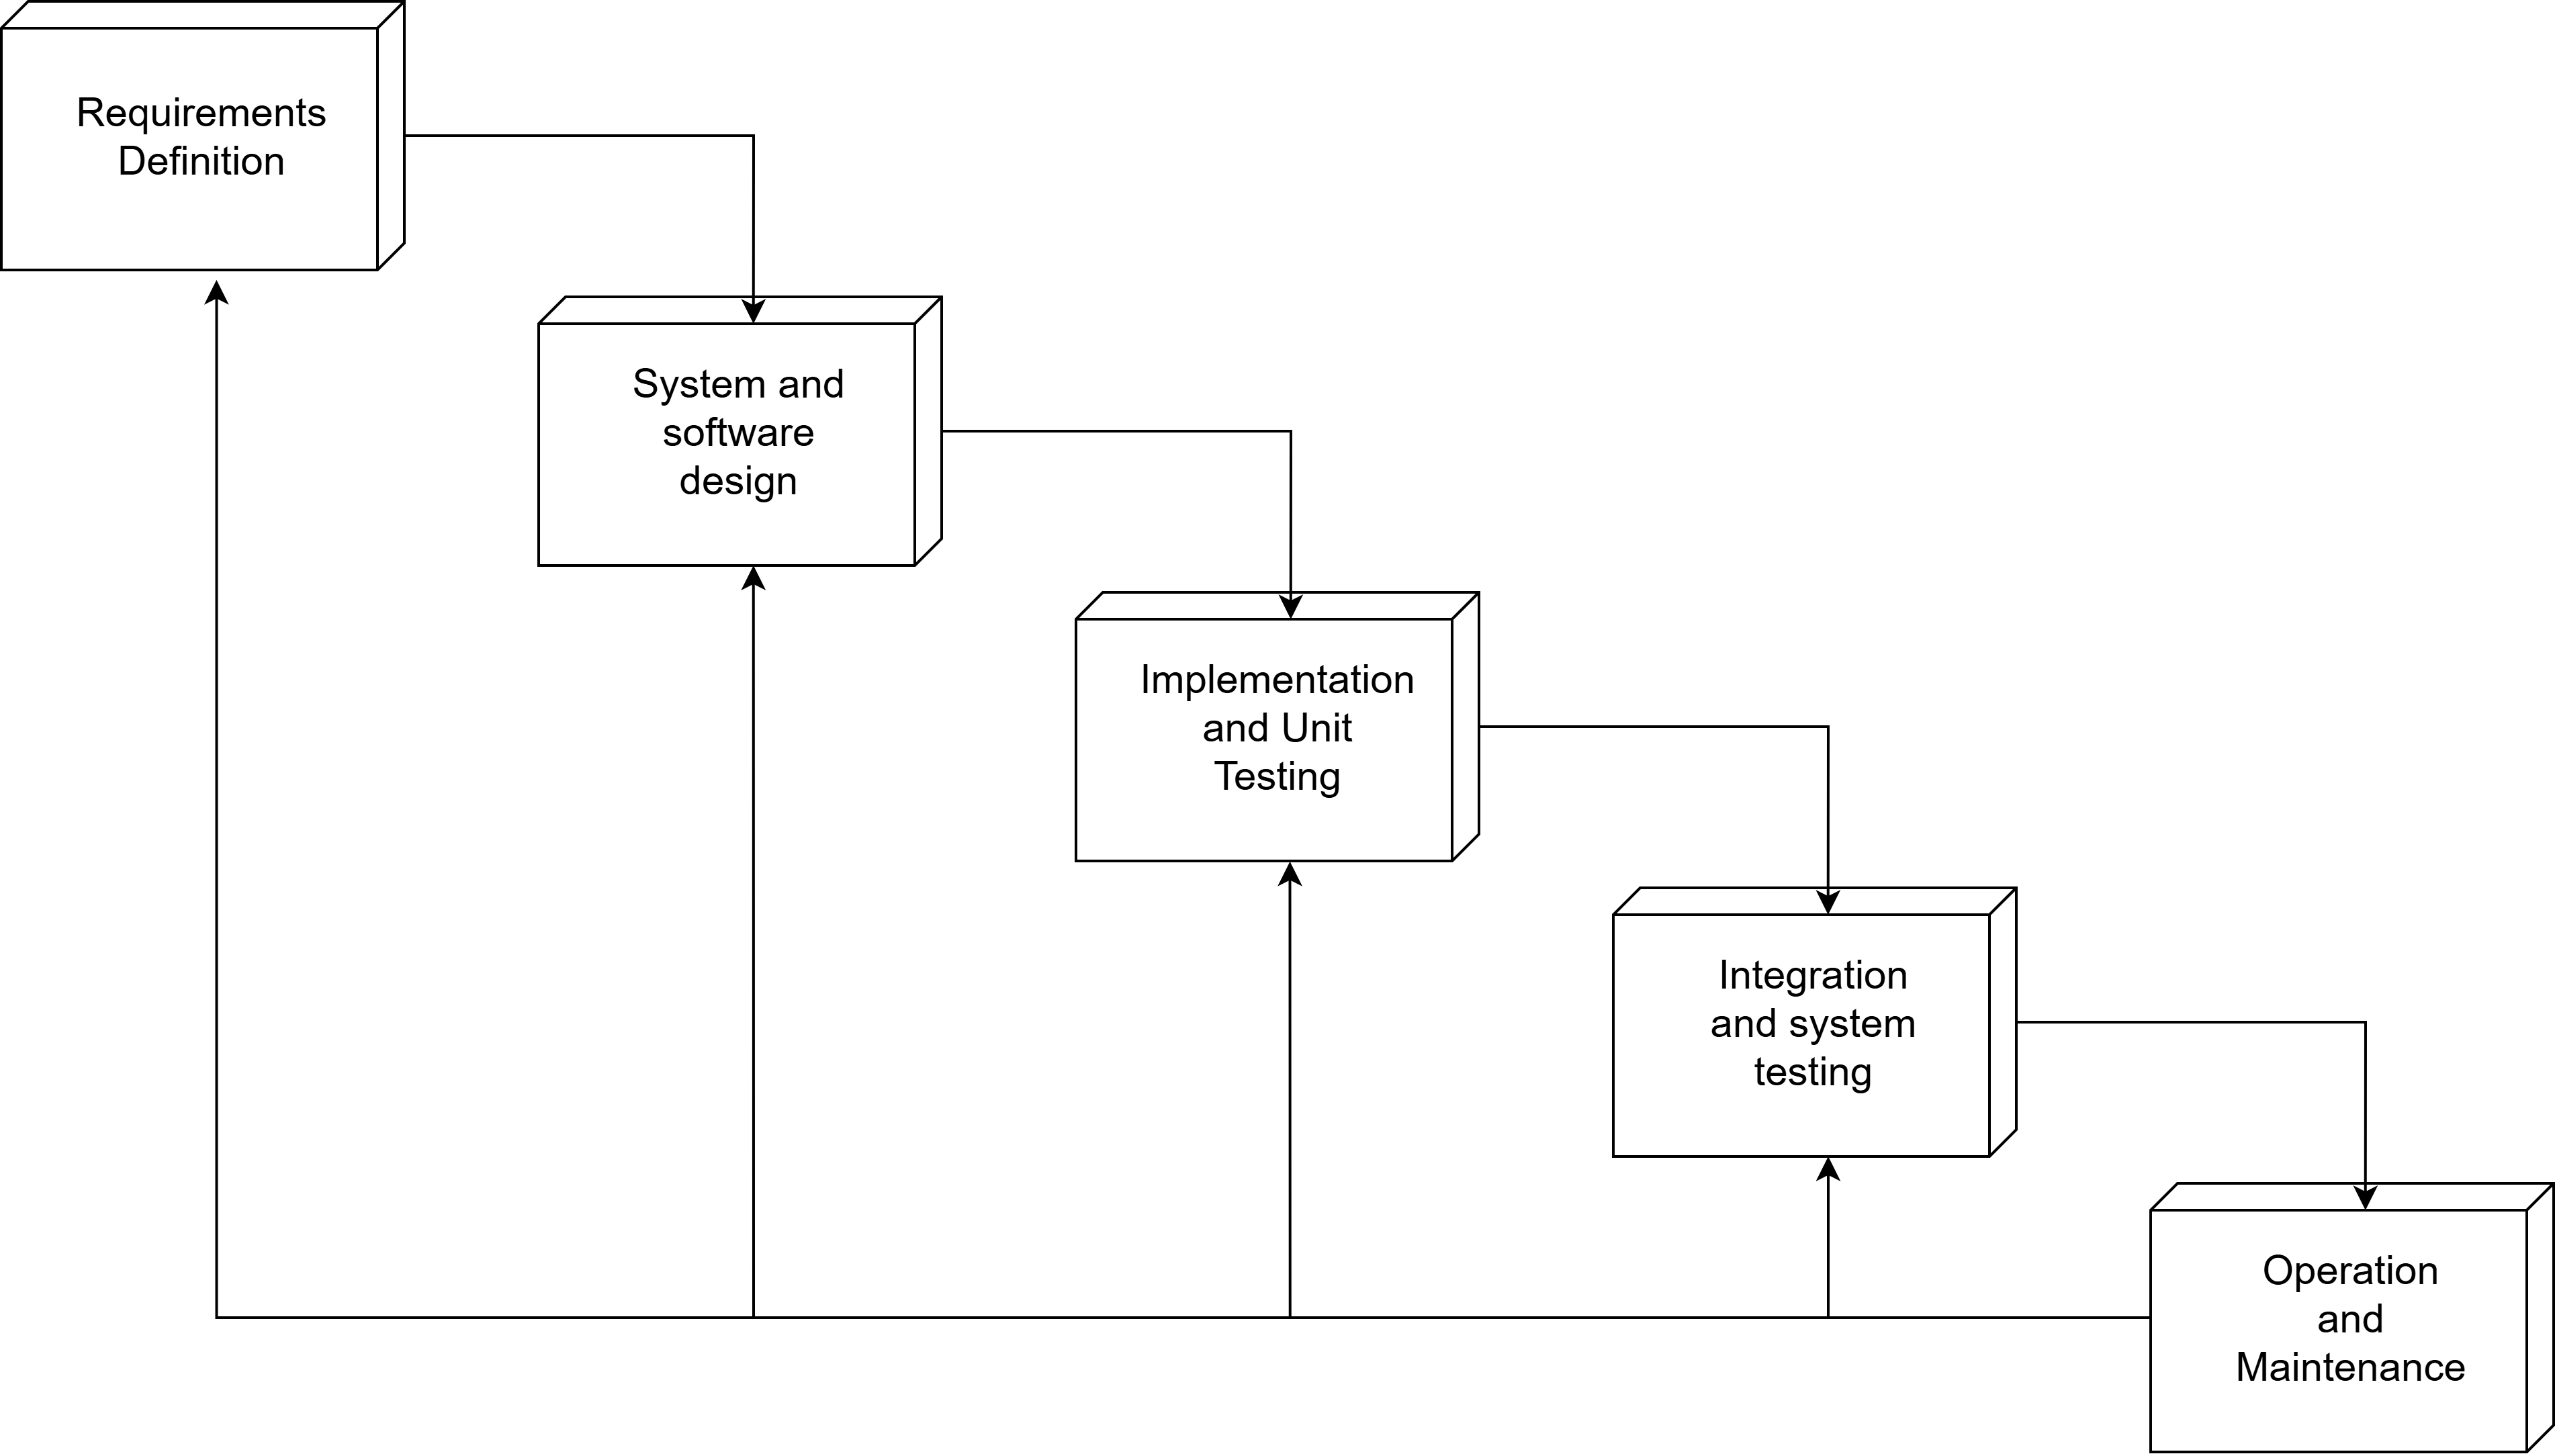
\includegraphics[width=.8\linewidth]{the_waterfall_model.png}
\caption{Figure 2- Depicts the Waterfall Model}
\label{fig:waterfall}
\end{figure}
\textbf{How Netflix Would Be Developed Using Waterfall:}
\begin{enumerate}
    \item \textbf{Phase 1:Requirements Definition} – All system requirements are defined at once in this phase. This includes defining user authentication, content streaming capabilities, personalized recommendations, and offline viewing. In short, developers try to gather any and all requirements in this stage. Since changes are difficult to implement later, this is very important and exhaustive documentation is required at this stage.
    \item \textbf{Phase 2: System \& Software Design} – A complete architecture is developed or produced in this phase. Including all the database structures and whatever big data models that are to be applied. API endpoints, and server infrastructure on AWS is developed all at once in this stage, again since further changes are very difficult in the waterfall model. Every aspect of the system is carefully mapped out before development begins.
    \item \textbf{Phase 3: Implementation} – Developers begin coding the entire system in one go, this has to be done since changes are tough to make, so they follow the previously defined architecture. No changes to the requirements are permitted, and development follows a sort of linear path, as shown in \emph{Figure 2}.
    \item \textbf{Phase 4: Integration and System Testing} – After development is completed, the entire system undergoes integration and rigorous testing. Integration becomes a crucial part in this process since, they have to be very fluid with integrating it properly so it runs everywhere without any hassle, otherwise the millions of people using it will be affected. Now the testing phase includes functional testing, performance testing, and security testing. Since all components are built at once, identifying and fixing bugs can be time-consuming.
    \item \textbf{Phase 5: Operation and Maintenance} – The fully developed streaming platform is deployed to production. Now this can be localised, for example to a specific country, region or even the whole world. This marks the system’s release, and users can now access Netflix. Any bugs or issues discovered post-launch are addressed during the maintenance. However, because in this model new changes require extensive planning and reimplementation, updates take a long time to roll out and overall, we can see how this is very inefficient, especially for a data-driven and dynamic organization such as Netflix.
\end{enumerate}
\newpage
\textbf{Suitability for Netflix:}
\begin{enumerate}
    \item \textbf{Pros:}
    \begin{itemize}
        \item Well-documented and structured approach. It sort of ensures clarity in development.
        \item Separate and properly defined phases simplify project management. It sort of Distributes the management on each step.
        \item Suitable for smaller, well-defined projects with minimal expected changes.
    \end{itemize}
    \item \textbf{Cons:}
    \begin{itemize}
        \item Majorly it lacks flexibility for rapidly changing user needs.
        \item If issues are discovered later on, it can cause significant delays.
        \item The long development cycles that we discussed, make it unsuitable for continuous updates.
    \end{itemize}
    \item \textbf{Verdict:} Not suitable, as Netflix requires frequent updates, rapid feature deployment, and adaptability to its evolving user preferences.
\end{enumerate}

\subsection{\textcolor{Blue}{Incremental Development Model}}
\begin{figure}[tbhp]
\centering
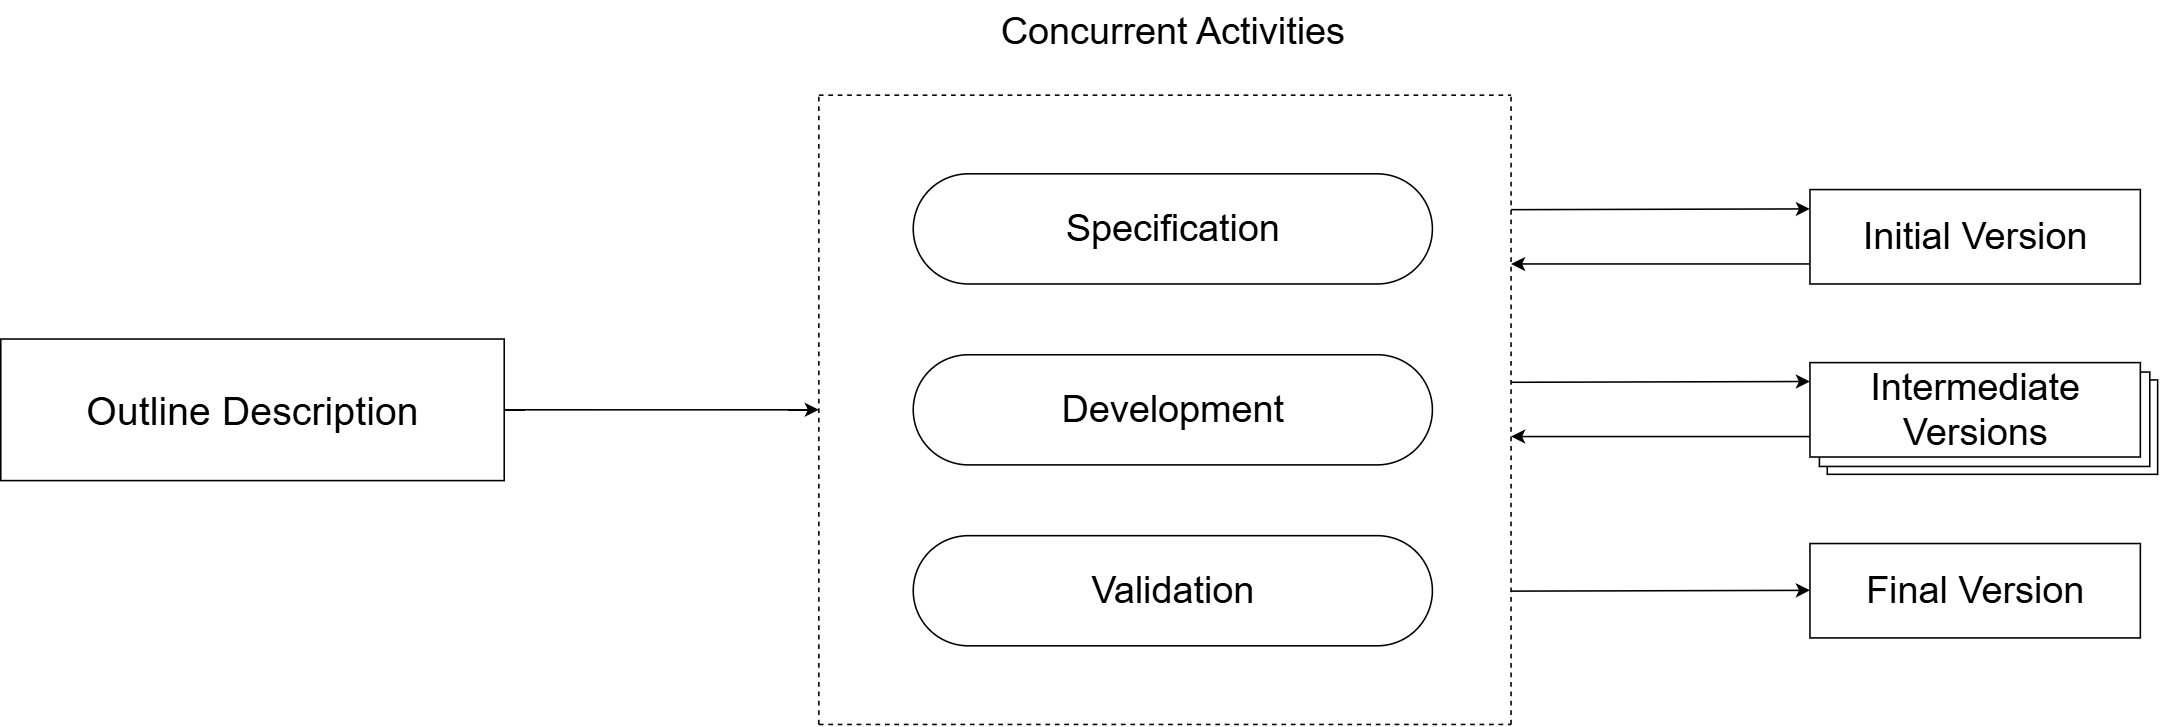
\includegraphics[width=.8\linewidth]{Incremental Development Model.png}
\caption{Figure 3- represents the Incremental Development Model}
\label{fig:incremental}
\end{figure}
\textbf{How Netflix Uses Incremental Development:}
\begin{enumerate}
    \item \textbf{Phase 1: Planning and Initial Requirements} – This model is a priority-based model. It is variable and can be revised multiple times. It is clearly represented in Figure 3. The development team identifies high-priority features, such as user authentication, video playback, and recommendation algorithms. These are the core components for Netflix especially. Only essential requirements for the first iteration are finalized, leaving room for future updates. This causes less complicated and piled development. I also feel it gives more head room to developers. 
    \item \textbf{Phase 2: Feature-wise Development} – Instead of developing the entire system at once, Netflix will be able to continuously releases new features. Now for example, it can improve the recommendation algorithms, have new content categories, and enhanced offline viewing. Each feature undergoes design, development, testing, and deployment in separate cycles, and each of it can be visited again, changes can be made. It makes it very sophisticated, speaking in terms of development.
    \item \textbf{Phase 3: Continuous User Feedback} – Each increment is deployed to beta users who provide feedback through usage patterns and explicit ratings. This becomes very helpful for Netflix since, if there are any bugs or inconveniences, it won’t affect its actual users. Developers analyse this feedback and make necessary adjustments before launching the next increment. Now, feedback is also taken through its regular users too. But the idea is to reduce the inconvenience caused to them and to provide them with a reliable platform.
    \item \textbf{Phase 4: System Testing and Refinement} – Every new feature or update undergoes extensive testing. Each development phase can be visited again, developers can add as many changes as they want, like we have already discussed. This including performance analysis, bug fixes, and security assessments. Automated pipelines are used, which is an awesome way to ensure continuous integration and testing.
    
    \item\pagebreak \textbf{Phase 5: Deployment and Monitoring} – Features are released to production in batches. By batches, I mean it can be released to a specific localized zone, a country, etc. This ensures minimal downtime. Something called an A/B testing is often used to compare different versions of a feature before full-scale deployment. This can really help Netflix with seamless user experience.
    \item \textbf{Phase 6: Iteration and Maintenance} – Now, as we discussed, this is an iterative process. It’s like a cycle that repeats as developers refine existing features, resolve any user-reported issues, and also when they introduce new functionalities to the platform, which is done based on the ever-changing user needs.
\end{enumerate}
\textbf{Suitability for Netflix:}
\begin{enumerate}
    \item \textbf{Pros:}
    \begin{itemize}
        \item Faster time-to-market with incremental feature releases, since developments are pushed in an efficient way
        \item It provides a quick adaptation to the changing user needs.
        \item The Continuous testing that we have discussed, ensures a high reliability and better performance overall for Netflix.
        \item This makes it easily scalable especially for a platform like Netflix and it also supports cloud-based microservices architecture, on which Netflix is currently based on.
    \end{itemize}
    \item \textbf{Cons:}
    \begin{itemize}
        \item Requires effective integration strategies to avoid system conflicts, which makes it a little more complicated.
        \item Needs a strong version control mechanisms to manage multiple development branches, and how they merge together.
        \item They can become complex if too many features are being worked on or developed simultaneously.
    \end{itemize}
    \item \textbf{Verdict:} \textcolor{Blue}{Highly suitable} for such a large-scale, evolving platform like Netflix, as it supports continuous and almost seamless updates and user-driven enhancements.
\end{enumerate}

\subsection{\textcolor{Blue}{Spiral Model}}
\begin{figure}[h]
\centering

\includegraphics[width=.65\linewidth]{Spiral Model.png}
\caption{Figure 4- Represents the Spiral Model}
\label{fig:spiral}
\end{figure}
\newpage
\textbf{How Netflix Would Be Developed Using Spiral:}
\begin{enumerate}
    \item \textbf{Phase 1: Risk Analysis and Prototyping} – Prior to deploying a significant feature maybe like AI-powered recommendations, etc, Netflix analyses the risks surrounding it. This includes algorithm biases, data security threats, and performance overhead. In a spiral model it is feasible to develop small scale prototypes first, before proceeding to develop on a full scale. This makes it separated and better maintained, and is efficient when it comes to testing.
    \item \textbf{Phase 2: Concept Validation and Refinement} – Once they test the prototype, Netflix takes in preliminary data and refines the design of the feature. This is generally done for many times, until a satisfactory and stable version can be launched. This iterative process helps validate the feature against technical limitations and business objectives. Overall, it makes the process provide quality outputs.
    \item \textbf{Phase 3: Development and Testing} – The features are built and tested in multiple cycles. Developers follow this iterative approach; they make changes based on risk assessment and the early feedback that they get from the beta users before the feature actually reaches full-scale deployment.
    \item \textbf{Phase 4: Validation and Security Testing} – The features are developed and tested in many iterations based on risk assessment and the initial feedback, changes are made, and the feature is gradually rolled out to higher-scale environments until full deployment. This is important for all of the complex features such as the machine learning models, personalization features, and data privacy regulations. Some of which are core components for Netflix.
    \item \textbf{Phase 5: Gradual Deployment} – The developed feature is initially deployed to few users, as discussed previously, some software use something like a beta version of their application, so that some people can now test their updates before it goes to all users. Real-world performance is monitored, and adjustments will be made before scaling the deployment to a larger audience.
    \item \textbf{Phase 6: Refinement and Continuous Improvement} – By having a strong network of beta testers, as discussed in the previous phase, developers use real-time analytics and user insights to refine the feature further. This cycle will repeat for future improvements, ensuring a sort of innovation that’s happening while the app is running live and used by millions around the world, while minimizing the risks.
\end{enumerate}
\textbf{Suitability for Netflix:}
\begin{enumerate}
    \item \textbf{Pros:}
    \begin{itemize}
        \item The iterations help a stronger risk management which in turn ensures robust system development.
        \item Iterative improvements also help refine complex features like AI-driven personalization.
        \item Suitable for the large-scale, high-risk functionalities such as the security upgrades and algorithm-driven recommendations.
    \end{itemize}
    \item \textbf{Cons:}
    \begin{itemize}
        \item It is expensive and time-consuming even for simple features, thus making it a little inefficient for such things.
        \item Requires highly skilled teams to develop using this model and assess risks accurately.
        \item Can be inefficient for routine updates that do not involve high-risk factors, and especially those which have minor fixes.
    \end{itemize}
    \item \textbf{Verdict:} Suitable for \textcolor{Blue}{high-risk features} for example, the security updates, AI-based recommendations, cloud infrastructure upgrades, etc but may not be necessary for routine feature development.
\end{enumerate}
\newpage
\subsection{Summary of Comparison}
\begin{table}[h]
    \centering
    \setlength{\tabcolsep}{10pt}
    \renewcommand{\arraystretch}{1.5}
    \resizebox{\textwidth}{!}{\begin{tabular}{|l|c|c|c|c|c|}
        \hline
        \textbf{SDLC Model} & \textbf{Flexibility} & \textbf{Risk Management} & \textbf{Time-to-Market} & \textbf{Cost} & \textbf{Suitability} \\
        \hline
        Waterfall & Low & Low & Slow & Medium & Not Suitable \\
        Incremental & High & Medium & Fast & High & Highly Suitable \\
        Spiral & High & High & Moderate & High & Suitable for High-Risk Features \\
        \hline
    \end{tabular}}
    \caption{Comparison of SDLC Models for Netflix}
\end{table}

\section{Requirements Engineering for Netflix}
Requirements engineering becomes a crucial part for Netflix. Everyone needs the platform to always deliver high performance, scalability, security and an amazing user experience. This has to be ensured through Netflix’s Software Development Lifecycle (SDLC). In this section, let’s dive into the core aspects of its requirements engineering practices, their significance and challenges associated with managing this for such a globally distributed and high-traffic platform.
\subsection{Functional Requirements}
By Functional requirements, I mean the specific behaviours and functionalities that it must support to meet the user expectations. Now, these will include:
\begin{itemize}
    \item \textbf{User Authentication \& Account Management:} Secure user registration and login using a platform called OAuth. In the present-day scenario, multi-factor authentication or MFA and social media sign-in is a must for users, for convenience and security both. Support for multiple user profiles under a single account, which has to also mean that users get personalised settings. For added security, it must include secure session management and logout functionality to prevent unauthorized access.
    \item \textbf{Content Streaming \& Playback} Adaptive bitrate streaming to provide the best video quality based on any network condition. Multi-device compatibility will allow seamless transitions between mobile, desktop, consoles, etc. A download feature which enables offline viewing with automatic content expiration (this follows the DRM compliances).
    \item \textbf{Recommendation System} AI-based content recommendations based on viewing history, preferences and how the user behaves. Also, as mentioned earlier, A/B testing and ML models can be used for dynamic algorithm adjustment.
    \item \textbf{Search \& Navigation} Efficient search filters based on genres, ratings and overall user preference and personalized UI/UX.
    \item \textbf{Payment \& Subscription Management} Support for different payment methods like credit/debit cards, UPI, PayPal, etc. Automated subscription renewal systems can also be included.
    \item \textbf{Content Management System} Backend or an admin interface for managing and updating content metadata, genres, and subtitles. A system for reviewing and approving newly uploaded content before publication.
    \item \textbf{Parental Controls} Age-restricted content management and customizable parental controls. It can have a PIN-based access for mature content.
    \item \textbf{User Analytics \& Insights} Collection of user engagement data for personalization and marketing strategies. This data can be anything like watch time, drop-off rates and content popularity. Integrating predictive analytics to enhance the experience is also possible.
\end{itemize}
\newpage
\subsection{Non-Functional Requirements}
\begin{itemize}
    \item \textbf{Scalability} The system must handle millions of concurrent users without a drop in performance. AWS Auto Scaling and Load balancing can be used to dynamically allocate resources based on demand.
    \item \textbf{Availability} A decent uptime can be achieved through multi-region AWS deployment. Redundant servers to prevent outages, etc.
    \item \textbf{Security} End-to-end encryption like TSL/SSL encryptions, secure user authentication mechanisms which must include biometric/CAPTCHA verification and fraud detection with periodic security and penetration testing.
    \item \textbf{Performance} Low latency for streaming and quick content buffering. It can use Content Delivery Networks (CDNs) like AWS CloudFront for faster content delivery.
    \item \textbf{Compliance \& Legal Considerations} Adherence to GDPR, DMCA, and copyright laws. Digital Rights Management (DRM) to prevent unauthorized content distribution.
    \item \textbf{Maintainability \& Upgradability} Has to include support for continuous deployment and infrastructure upgrades.
\end{itemize}

\subsection{Requirements Validation Strategy}
It ensures that all functional and non-functional specs align with Netflix’s objectives. It employs various techniques to validate the software requirements:
\begin{itemize}
    \item \textbf{Stakeholder Reviews} Collaborating with business teams, developers, and end-users can help in refining requirements.
    \item \textbf{Prototyping \& A/B Testing} Testing UI/UX at an early stage and data-driven decisions can be taken based on user behaviour.
    \item \textbf{Automated Testing \& CI/CD Pipelines} Integration of unit, functional, and regression testing can be done to ensure compliance with various regulations.
    \item \textbf{Security Audits} Continuously assessing vulnerability and penetration testing to make it secure and meet all the security regulations.
    \item \textbf{User Feedback Loops} Collection of real-time analytics helps it a lot to adapt to its evolving customer needs.
\end{itemize}

\subsection{Challenges in Requirements Validation}
Despite a good structured validation approach, Netflix faces challenges in requirements validation:
\begin{itemize}
    \item \textbf{Dynamic User Expectations: } Trends tend to change constantly in entertainment consumption as we all know.
    \item \textbf{Global Compliance Issues: } Adapting to different regional content laws and licensing agreements becomes a tedious job.
    \item \textbf{Scalability \& Performance Bottlenecks: } Handling peak traffic loads and maintaining seamless service across diverse network conditions is difficult speaking of the infrastructure.
    \item \textbf{AI Bias in Personalization: } Ensuring fairness and inclusivity in recommendations. Sometimes it can over-prioritize specific genres or demographics.
    \item \textbf{Content Piracy \& Security Threats: } There has been a rising threat of piracy platforms and constantly evolving risks in digital rights management.
\end{itemize}
\newpage
\section{Conclusion}
Netflix, as we know is a continuously evolving platform. Based on our understanding from this paper, we can conclude that it benefits most from Incremental Development for \textcolor{Blue}{rapid feature deployment} and Spiral Model for \textcolor{Blue}{high-risk features}. The Waterfall model is not suitable due to its rigid structure.
It has a very effective requirements engineering process that ensures that Netflix meets both functional and non-functional demands.

\section{References}
\begin{thebibliography}{9}
    \bibitem{pressman} Sommerville, I. (2015). \textit{Software Engineering} (10th Edition).
    \bibitem{netflix_blog} Netflix Technology Blog - \url{https://netflixtechblog.com/}
    \bibitem{wikipedia} Wikipedia – Netflix; as edited on 3rd February 2025  - \url{https://en.wikipedia.org/wiki/Netflix}
    \bibitem{aws} AWS Whitepapers on Netflix’s cloud infrastructure.
\end{thebibliography}

\end{document}
